\section{Numerical Experiments}\label{sec:exp} 
We  now show via experiments that gates indeed play a central role in DNNs with ReLU. For this we use the DGN setup (\Cref{fig:ablation}) to create models in the $4$ regimes namely DL, FL, FR-II and FR-DI. In each of the $4$ regimes, we create  combinatorially many models via a) permutation of the layers when the copied from the feature to the value network, and b) setting the input to the value network to $\mathbf{1}$ (in training and testing), i.e., a tensor with all its entries to be $1$. We observe that in all the $4$ regimes, the models are robust to the combinatorial variations (i.e., $48$ different models, see \Cref{tb:ablation}).

\textbf{Setup:} Datasets are MNIST and CIFAR-10. For CIFAR-10, we use \Cref{fig:ablation} with $3\times 3$  windows and $128$ filters in each layer. For MNIST, we use FC instead of the convolutional layers.  All the FC-DNNs and CNNs are trained with `\emph{Adam}'  \cite{adam} (step-size $=3\cdot 10^{-4}$ , batch size $=32$). We use $\beta=10$ in the DL regime.

\textbf{Reporting of Statistics:} The results are in \Cref{tb:ablation}. For FC-DNN and CNN, in each of the $4$ regimes, we train $48= 2 (\xv=x / \xv=\mathbf{1}) \times 24(\text{layer permutations})$ models. Each of these models are trained to almost $100\%$ accuracy and the test performance is taken to be the best obtained in a given run. Each of the $48$ models is run only once, and the performance is averaged across all the $48$ models.
\begin{figure}
\begin{minipage}{0.6\columnwidth}
\resizebox{\columnwidth}{!}{
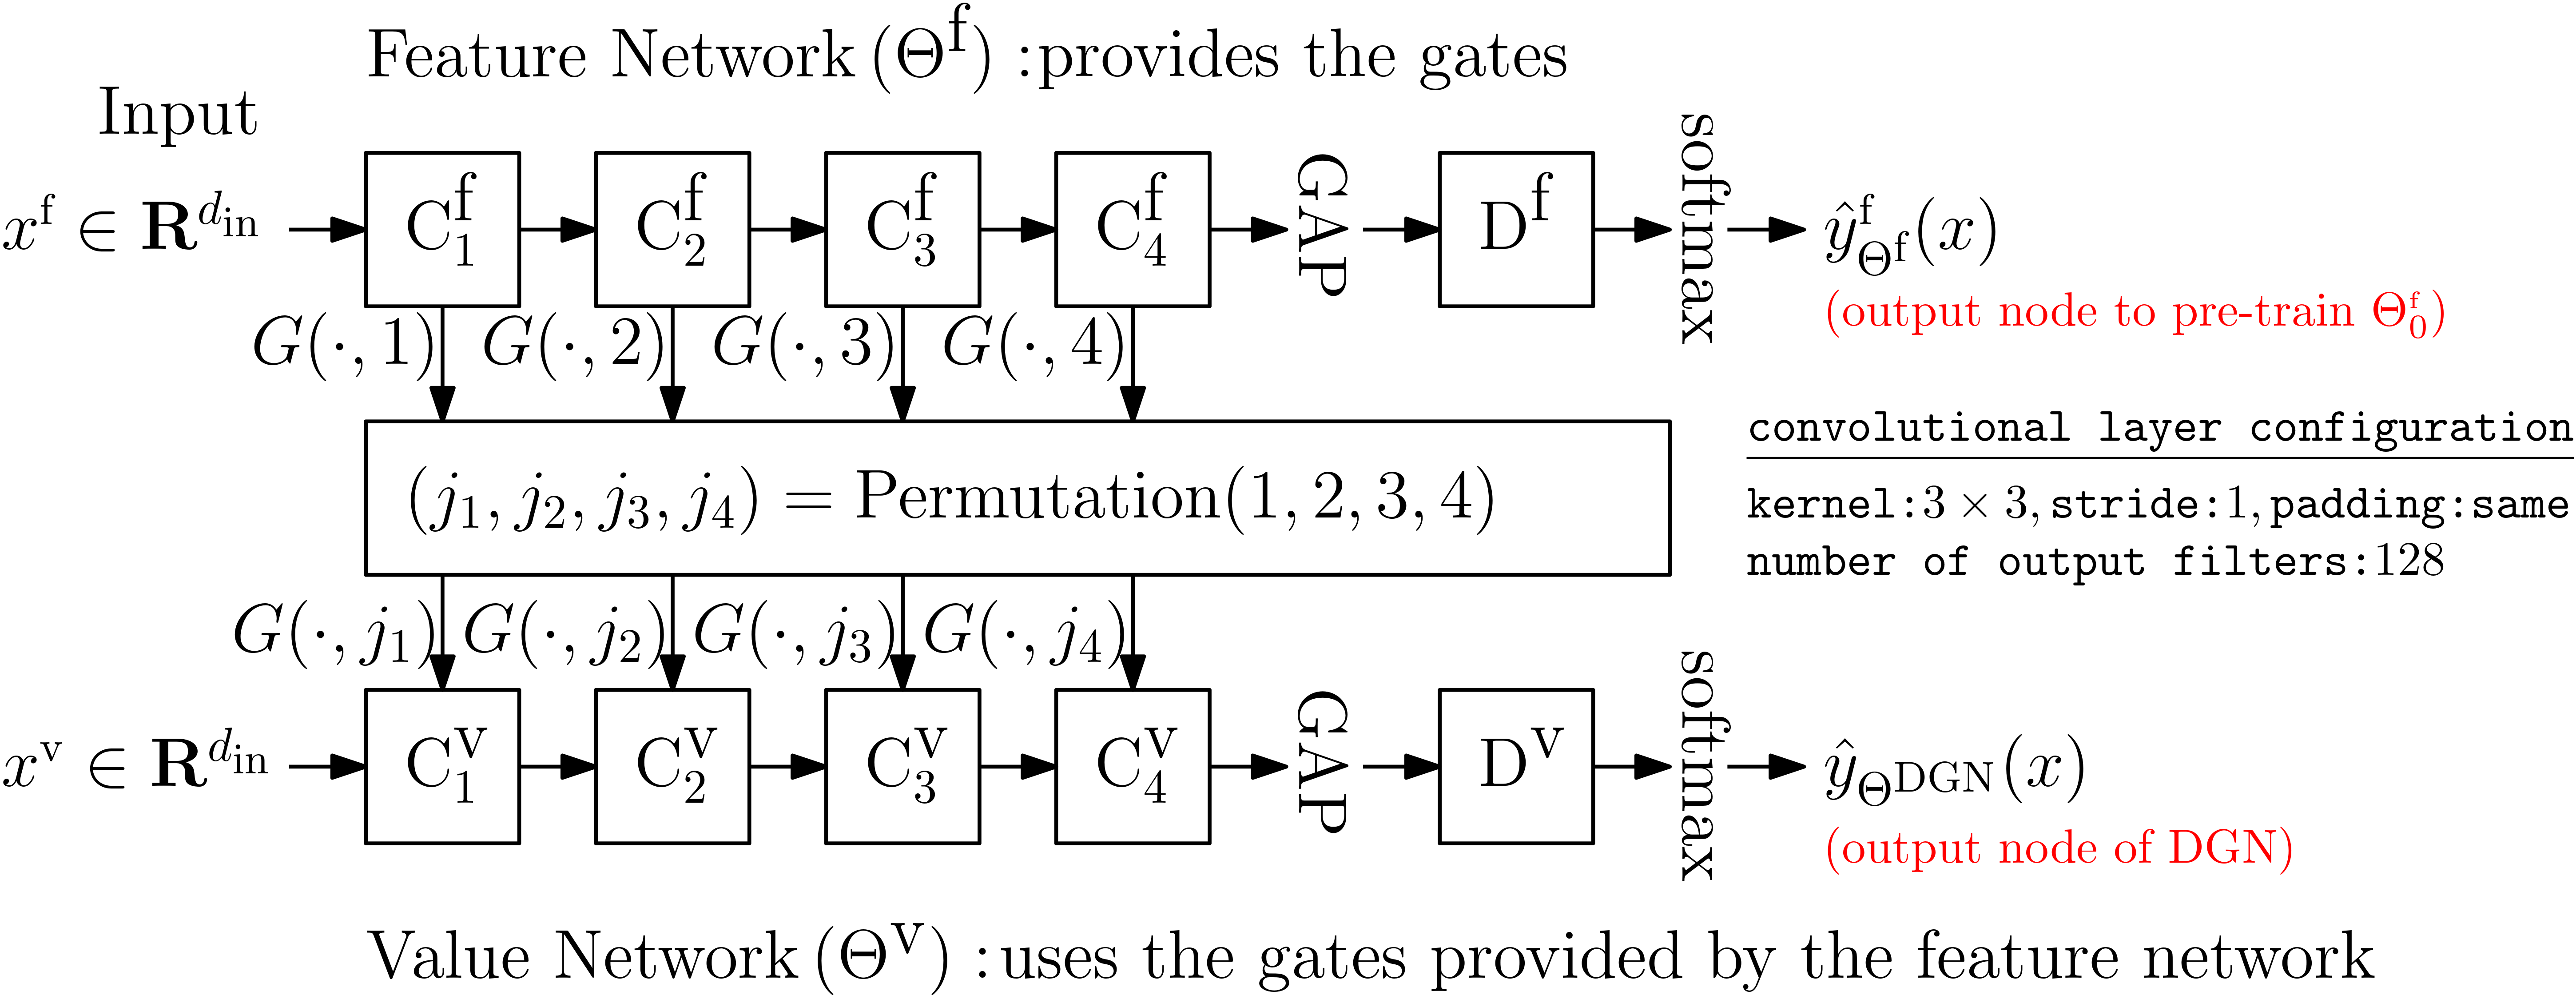
\includegraphics[scale=0.5]{figs/ablation.png}
}
\end{minipage}
\begin{minipage}{0.3\columnwidth}
\resizebox{\columnwidth}{!}{
\begin{tabular}{|p{1.75cm}|c|c|c|c|c|}\hline
& FR-II &FR-DI & DL& FL& ReLU\\\hline
\centering{FC (MNIST)} &$94.1\%$  &$94.1\%$  &$98.1\%$ &$98.6\%$ &$98.5\%$\\\hline
\centering{CNN (CIFAR-10)}&$67.5\%$ &$67.6\%$   &$77.6\%$ &$79.4\%$ &$80.4\%$\\\hline
\end{tabular}
}
\end{minipage}
\caption{\small{$\textrm{C}_i^{\text{f}},\textrm{C}_i^{\text{v}},i\in[4]$ are the convolutional layers, which are followed by \emph{global-average-pooling} (GAP) layer then by a dense layer ($\textrm{D}^{\text{f}}$/$\textrm{D}^{\text{v}}$), and a softmax layer to produce the final logits.}} %`R',  `L', `T' and `NT' stand for random, learnt, trainable and non-trainable respectively.}}
\label{fig:ablation}
\end{figure}
\begin{comment}
\FloatBarrier
\begin{table}[h]
\centering
\begin{tabular}{|p{1cm}|p{1.6cm}|p{1.7cm}p{0.001cm}|}\hline
&\centering{FC (MNIST)}& \centering{CNN (CIFAR-10)}& \\\hline
FR-II& \centering$94.1\%$ & \centering$67.5\%$& \\\hline
FR-DI& \centering$94.1\%$ & \centering$67.6\%$& \\\hline
DL& \centering$98.1\%$ & \centering$77.6\%$&\\\hline
FL& \centering$98.6\%$ & \centering$79.4\%$&\\\hline
ReLU& \centering$98.5\%$ & \centering$80.4\%$&\\\hline
\end{tabular}
\caption{Shows test accuracies in each of the $4$ different regimes. In all the $4$ regimes (FC as well as CNN) the results averaged over the $48$ different modes. In all cases, standard deviation was less than $0.5\%$.}
\end{table}
\end{comment}
\begin{table}



\caption{Shows test accuracies in each of the $4$ different regimes.  \textbf{In all the $\mathbf{4}$ regimes (FC as well as CNN) the results in this table are averaged over the $\mathbf{48}$ different models ($\mathbf{24\times 2}=48$ models). In all cases, standard deviation was less than $\mathbf{0.5\%}$ and hence not mentioned in the table}.}
\label{tb:ablation}
\end{table}


$\bullet$ \textbf{Result Discussion:}  Recall that in regimes FR-II and FR-DI the gates are fixed and random, and only $\Tv$ are trained. In DL regime, both $\Tf$ and $\Tv$ are trained, and FL regime $\Tf$ is pre-trained and fixed, and only $\Tv$ is trained. In the following discussion, we compare the performance of the models in various regimes, along with the performance of CNTK of \citet{arora2019exact} ($77.43\%$ in CIFAR-10) and the performance of standard DNN with ReLU.  The main observations are listed below (those by \citet{npk} are also revisited for the sake of completeness). 

\indent\quad $1.$ \emph{Decoupling:} There is no performance difference between FR-II and FR-DI.% i.e., the decoupling the gates from the weights did not affect the performance in practice. 
Further, decoupled learning of gates (DL) performs significantly better than fixed random gates (FR), and the gap between standard DNN with ReLU and DL is less than $3\%$. This marginal performance loss seems to be worthy trade off for fundamental insights of \Cref{th:main} under the decoupling assumption.

\indent\quad $2.$ \emph{Recovery:} The fixed learnt regime  (FL) shows that using the gates of a pre-trained ReLU network, performance can be recovered by training the NPV. Also, by interpreting the input dependent component of a model to be the features and the input independent component to be the weights, it makes sense to look at the gates/NPFs as the hidden features and NPV as the weights.% (which can be re-trained).

\indent\quad $3.$ \emph{Random Gates:} FR-II does perform well in all the experiments (note that for a $10$-class problem, a random classifier would achieve only $10\%$ test accuracy). Given the observation that the gates are the true features, and the fact that is there no learning in the gates in the fixed regime, and the performance of fixed random gates can be purely attributed to the in-built structure.

\indent\quad $4.$ \emph{Gate Learning:} We group the models into three sets where $S_1=\{$ ReLU, FL , DL$\}$, $S_2=\{$ FR$\}$ and $S_3=\{$ CNTK $\}$, and explain the difference in performance due to gate learning.
 $S_2$ and $S_3$ have no gate learning. However,  $S_3$ due to its infinite width has better averaging resulting in a well formed kernel and hence performs better than $S_2$ which is a finite width. Thus, the difference between $S_2$ and $S_3$ can be attributed to finite versus infinite width. Both $S_1$ and $S_2$ are finite width, and hence, conventional feature learning happens in both $S_1$ and $S_2$, but, $S_1$ with gate learning is better ($77.5\%$ or above in CIFAR-10) than $S_2$ ($67\%$ in CIFAR-10) with no gate learning. Thus neither finite width, nor the conventional feature learning explain the difference between $S_1$ and $S_2$. Thus, `gate learning' discriminates the regimes $S_1, S_2$ and $S_3$ better than the conventional feature learning view.

\indent\quad $5.$ \emph{Permutation and Constant Input:} The performance (in all the $4$ regimes) is  robust to `all-ones' inputs. Note that in the `all-ones' case, the input information affects the models only via the gates. Here, all the entries of the input Gram matrix are identical, and the NPK depends only on the base kernels. The performance (in all the $4$ regimes) is also robust to permutation of the layers. This can be attributed to the product $\Pi_{l=1}^{(d-1)} H^{\text{lyr}}_{l,\Theta}$ of the layer level base kernels being permutation invariant. A particularly striking example of robustness to permutations and constant input is presented in \Cref{fig:visual-permute}. Here,  we contrast the hidden layer outputs of a standard CNN with ReLU with $4$ layers, and that of a DGN which copies the gates from the standard CNN, but, reverses the gating masks when applying to the value network. Also, the value network of the DGN was provided with a fixed random input. Both the models achieve about $80\%$ test accuracy.  This suggests that visually interpreting the hidden layer outputs may not be meaningful.
\begin{figure}[h]
\begin{minipage}{0.3\columnwidth}
\resizebox{\columnwidth}{!}{
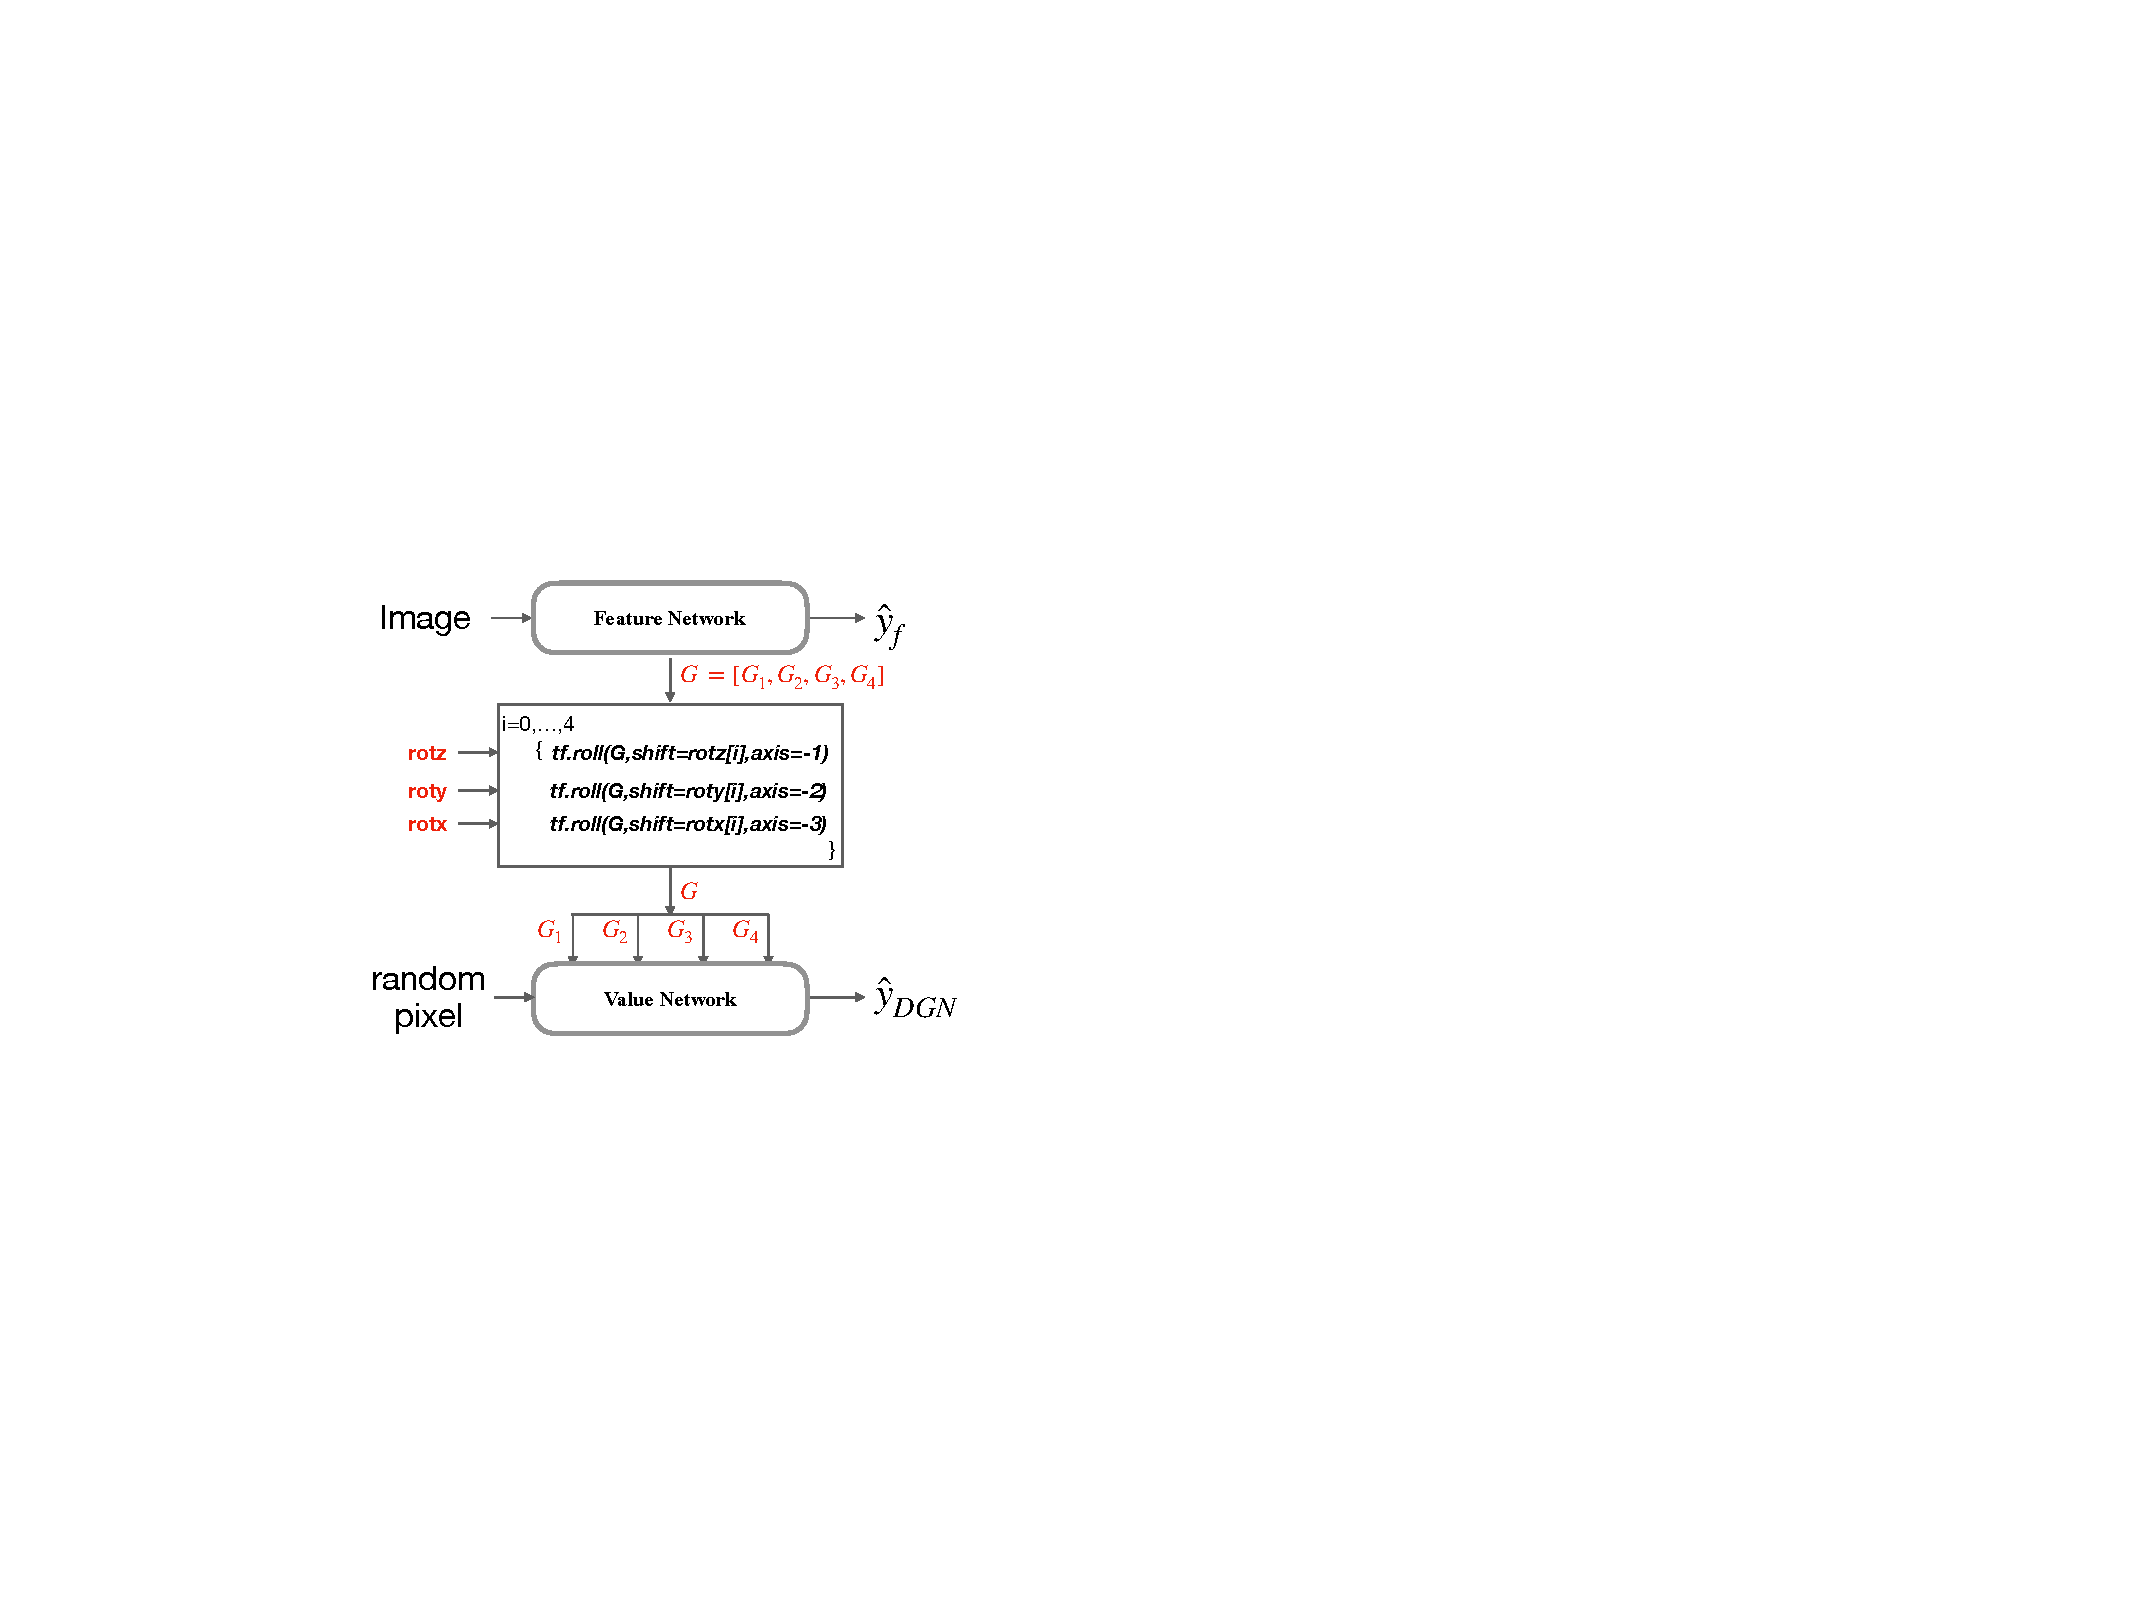
\includegraphics[scale=0.25]{figs/arbitrary_shift.pdf}
}
\end{minipage}
\begin{minipage}{0.68\columnwidth}
\resizebox{\columnwidth}{!}{
\begin{tabular}{cccccccccc}
&\Huge{Input}& \Huge{Layer 1, Filter 1}& \Huge{Layer 1, Filter 2}& \Huge{Layer 2, Filter 1}& \Huge{Layer 2, Filter 2}& \Huge{Layer 3, Filter 1}& \Huge{Layer 3, Filter 2}& \Huge{Layer 4, Filter 1}& \Huge{Layer 4, Filter 2}\\
\Huge{Feature Network}&\includegraphics{visual-iclr/images/horse.png}&
\includegraphics{images_neurips_2021/feature_network/layer_1_0.png}&
\includegraphics{images_neurips_2021/feature_network/layer_1_1.png}&
\includegraphics{images_neurips_2021/feature_network/layer_2_0.png}&
\includegraphics{images_neurips_2021/feature_network/layer_2_1.png}&
\includegraphics{images_neurips_2021/feature_network/layer_3_0.png}&
\includegraphics{images_neurips_2021/feature_network/layer_3_1.png}&
\includegraphics{images_neurips_2021/feature_network/layer_4_0.png}&
\includegraphics{images_neurips_2021/feature_network/layer_4_1.png}\\
\Huge{Value Network}&\includegraphics{images_neurips_2021/allones.png}&
\includegraphics{images_neurips_2021/value_network//layer_1_0.png}&
\includegraphics{images_neurips_2021/value_network//layer_1_1.png}&
\includegraphics{images_neurips_2021/value_network//layer_2_0.png}&
\includegraphics{images_neurips_2021/value_network//layer_2_1.png}&
\includegraphics{images_neurips_2021/value_network//layer_3_0.png}&
\includegraphics{images_neurips_2021/value_network//layer_3_1.png}&
\includegraphics{images_neurips_2021/value_network//layer_4_0.png}&
\includegraphics{images_neurips_2021/value_network//layer_4_1.png}
\end{tabular}
}

\end{minipage}
\caption{Top (Standard CNN): First image on the left is the input image and the next $8$ images are outputs of $2$ filters in each of the $4$ layers. Bottom (DGN with gates of the top model applied in reverse order): First image on the left is the input to the value network and the next $8$ images are outputs of $2$ filters in each of the $4$ layers. Both models achieve a test accuracy of about $80\%$.}
\label{fig:visual-permute}
\end{figure}


\indent\quad $6.$ \emph{Gate Only Training:} In this setting, both value network and the feature network are initialised at random. However, only the feature network is trained and the value network weights are kept fixed. We observe about $65\%$ test accuracy on CIFAR-10 by just training the gates. This experiment can be interpreted as tuning the gates in such a manner to select the right sub-network of random weights.
 